\documentclass{standalone}
\usepackage{ tikz }
\usepackage{ xparse }
\usepackage{../../../macros}

\begin{document}
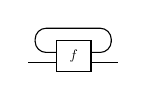
\begin{tikzpicture}[yscale=-1,x=1em,y=1.25em]
    
    \draw [rounded corners] (1.0,0) -- (1.0,0.3) -- (1.75,0.3);
    \draw [rounded corners] (1.0,0) -- (1.0,-0.4) -- (2,-0.4) -- (3.75,-0.4) -- (3.75,0);
    \draw [rounded corners] (3.75,0) -- (3.75, 0.3) -- (3, 0.3);
    \draw [] (0.75,0.6) -- (1.75,0.6);
    \draw [] (3, 0.6) -- (4,0.6);
    \node[draw, minimum height = 0.6em, minimum width = 1.25em, anchor = west, fill=white] at (1.75,0.4){\scalebox{0.5}{$f$}};

\end{tikzpicture}
\end{document}